\documentclass[1p]{elsarticle_modified}
%\bibliographystyle{elsarticle-num}

%\usepackage[colorlinks]{hyperref}
%\usepackage{abbrmath_seonhwa} %\Abb, \Ascr, \Acal ,\Abf, \Afrak
\usepackage{amsfonts}
\usepackage{amssymb}
\usepackage{amsmath}
\usepackage{amsthm}
\usepackage{scalefnt}
\usepackage{amsbsy}
\usepackage{kotex}
\usepackage{caption}
\usepackage{subfig}
\usepackage{color}
\usepackage{graphicx}
\usepackage{xcolor} %% white, black, red, green, blue, cyan, magenta, yellow
\usepackage{float}
\usepackage{setspace}
\usepackage{hyperref}

\usepackage{tikz}
\usetikzlibrary{arrows}

\usepackage{multirow}
\usepackage{array} % fixed length table
\usepackage{hhline}

%%%%%%%%%%%%%%%%%%%%%
\makeatletter
\renewcommand*\env@matrix[1][\arraystretch]{%
	\edef\arraystretch{#1}%
	\hskip -\arraycolsep
	\let\@ifnextchar\new@ifnextchar
	\array{*\c@MaxMatrixCols c}}
\makeatother %https://tex.stackexchange.com/questions/14071/how-can-i-increase-the-line-spacing-in-a-matrix
%%%%%%%%%%%%%%%

\usepackage[normalem]{ulem}

\newcommand{\msout}[1]{\ifmmode\text{\sout{\ensuremath{#1}}}\else\sout{#1}\fi}
%SOURCE: \msout is \stkout macro in https://tex.stackexchange.com/questions/20609/strikeout-in-math-mode

\newcommand{\cancel}[1]{
	\ifmmode
	{\color{red}\msout{#1}}
	\else
	{\color{red}\sout{#1}}
	\fi
}

\newcommand{\add}[1]{
	{\color{blue}\uwave{#1}}
}

\newcommand{\replace}[2]{
	\ifmmode
	{\color{red}\msout{#1}}{\color{blue}\uwave{#2}}
	\else
	{\color{red}\sout{#1}}{\color{blue}\uwave{#2}}
	\fi
}

\newcommand{\Sol}{\mathcal{S}} %segment
\newcommand{\D}{D} %diagram
\newcommand{\A}{\mathcal{A}} %arc


%%%%%%%%%%%%%%%%%%%%%%%%%%%%%5 test

\def\sl{\operatorname{\textup{SL}}(2,\Cbb)}
\def\psl{\operatorname{\textup{PSL}}(2,\Cbb)}
\def\quan{\mkern 1mu \triangleright \mkern 1mu}

\theoremstyle{definition}
\newtheorem{thm}{Theorem}[section]
\newtheorem{prop}[thm]{Proposition}
\newtheorem{lem}[thm]{Lemma}
\newtheorem{ques}[thm]{Question}
\newtheorem{cor}[thm]{Corollary}
\newtheorem{defn}[thm]{Definition}
\newtheorem{exam}[thm]{Example}
\newtheorem{rmk}[thm]{Remark}
\newtheorem{alg}[thm]{Algorithm}

\newcommand{\I}{\sqrt{-1}}
\begin{document}

%\begin{frontmatter}
%
%\title{Boundary parabolic representations of knots up to 8 crossings}
%
%%% Group authors per affiliation:
%\author{Yunhi Cho} 
%\address{Department of Mathematics, University of Seoul, Seoul, Korea}
%\ead{yhcho@uos.ac.kr}
%
%
%\author{Seonhwa Kim} %\fnref{s_kim}}
%\address{Center for Geometry and Physics, Institute for Basic Science, Pohang, 37673, Korea}
%\ead{ryeona17@ibs.re.kr}
%
%\author{Hyuk Kim}
%\address{Department of Mathematical Sciences, Seoul National University, Seoul 08826, Korea}
%\ead{hyukkim@snu.ac.kr}
%
%\author{Seokbeom Yoon}
%\address{Department of Mathematical Sciences, Seoul National University, Seoul, 08826,  Korea}
%\ead{sbyoon15@snu.ac.kr}
%
%\begin{abstract}
%We find all boundary parabolic representation of knots up to 8 crossings.
%
%\end{abstract}
%\begin{keyword}
%    \MSC[2010] 57M25 
%\end{keyword}
%
%\end{frontmatter}

%\linenumbers
%\tableofcontents
%
\newcommand\colored[1]{\textcolor{white}{\rule[-0.35ex]{0.8em}{1.4ex}}\kern-0.8em\color{red} #1}%
%\newcommand\colored[1]{\textcolor{white}{ #1}\kern-2.17ex	\textcolor{white}{ #1}\kern-1.81ex	\textcolor{white}{ #1}\kern-2.15ex\color{red}#1	}

{\Large $\underline{12n_{0094}~(K12n_{0094})}$}

\setlength{\tabcolsep}{10pt}
\renewcommand{\arraystretch}{1.6}
\vspace{1cm}\begin{tabular}{m{100pt}>{\centering\arraybackslash}m{274pt}}
\multirow{5}{120pt}{
	\centering
	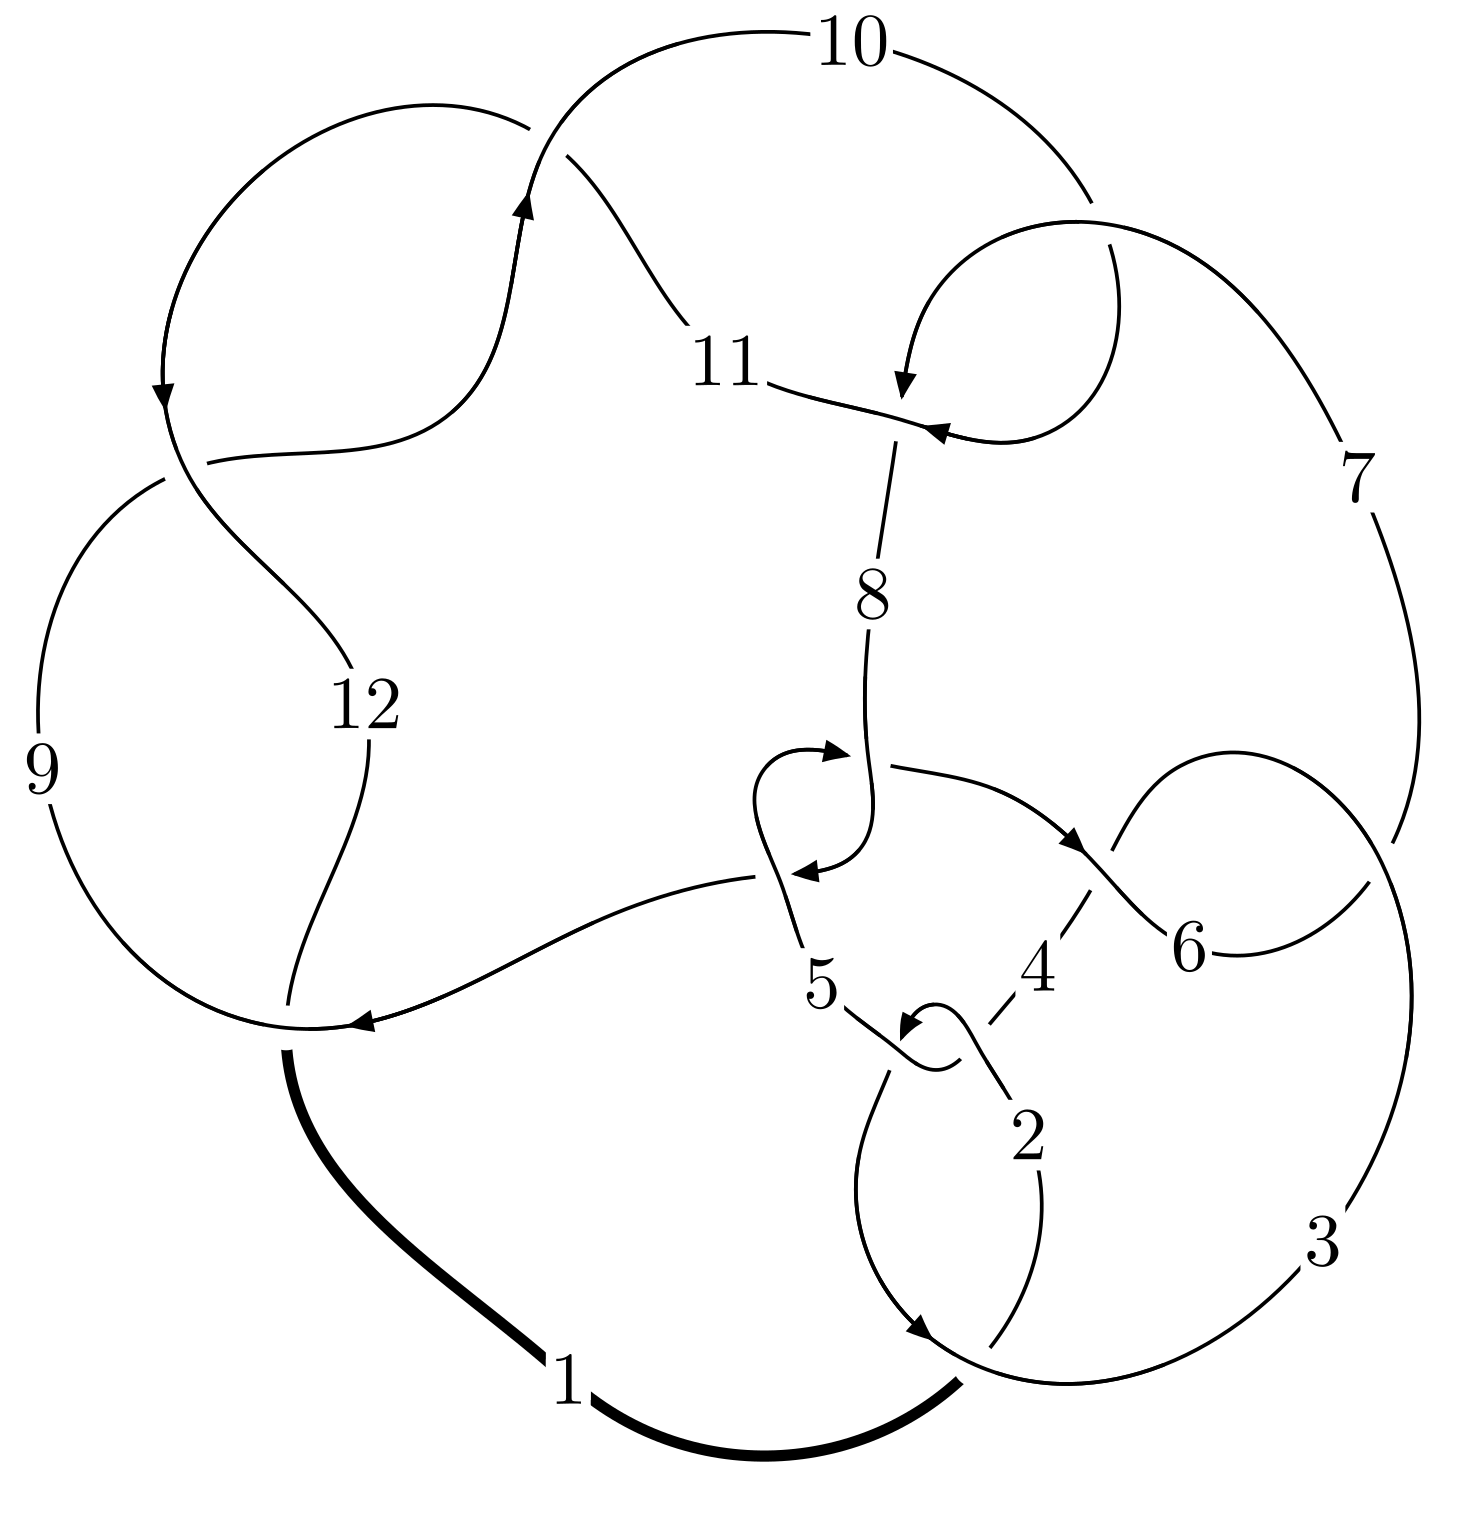
\includegraphics[width=112pt]{../../../GIT/diagram.site/Diagrams/png/2183_12n_0094.png}\\
\ \ \ A knot diagram\footnotemark}&
\allowdisplaybreaks
\textbf{Linearized knot diagam} \\
\cline{2-2}
 &
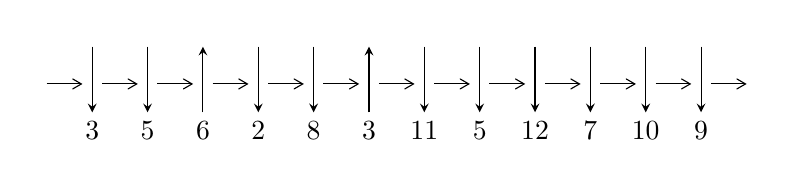
\begin{tikzpicture}[x=20pt, y=17pt]
	% nodes
	\node (C0) at (0, 0) {};
	\node (C1) at (1, 0) {};
	\node (C1U) at (1, +1) {};
	\node (C1D) at (1, -1) {3};

	\node (C2) at (2, 0) {};
	\node (C2U) at (2, +1) {};
	\node (C2D) at (2, -1) {5};

	\node (C3) at (3, 0) {};
	\node (C3U) at (3, +1) {};
	\node (C3D) at (3, -1) {6};

	\node (C4) at (4, 0) {};
	\node (C4U) at (4, +1) {};
	\node (C4D) at (4, -1) {2};

	\node (C5) at (5, 0) {};
	\node (C5U) at (5, +1) {};
	\node (C5D) at (5, -1) {8};

	\node (C6) at (6, 0) {};
	\node (C6U) at (6, +1) {};
	\node (C6D) at (6, -1) {3};

	\node (C7) at (7, 0) {};
	\node (C7U) at (7, +1) {};
	\node (C7D) at (7, -1) {11};

	\node (C8) at (8, 0) {};
	\node (C8U) at (8, +1) {};
	\node (C8D) at (8, -1) {5};

	\node (C9) at (9, 0) {};
	\node (C9U) at (9, +1) {};
	\node (C9D) at (9, -1) {12};

	\node (C10) at (10, 0) {};
	\node (C10U) at (10, +1) {};
	\node (C10D) at (10, -1) {7};

	\node (C11) at (11, 0) {};
	\node (C11U) at (11, +1) {};
	\node (C11D) at (11, -1) {10};

	\node (C12) at (12, 0) {};
	\node (C12U) at (12, +1) {};
	\node (C12D) at (12, -1) {9};
	\node (C13) at (13, 0) {};

	% arrows
	\draw[->,>={angle 60}]
	(C0) edge (C1) (C1) edge (C2) (C2) edge (C3) (C3) edge (C4) (C4) edge (C5) (C5) edge (C6) (C6) edge (C7) (C7) edge (C8) (C8) edge (C9) (C9) edge (C10) (C10) edge (C11) (C11) edge (C12) (C12) edge (C13) ;	\draw[->,>=stealth]
	(C1U) edge (C1D) (C2U) edge (C2D) (C3D) edge (C3U) (C4U) edge (C4D) (C5U) edge (C5D) (C6D) edge (C6U) (C7U) edge (C7D) (C8U) edge (C8D) (C9U) edge (C9D) (C10U) edge (C10D) (C11U) edge (C11D) (C12U) edge (C12D) ;
	\end{tikzpicture} \\
\hhline{~~} \\& 
\textbf{Solving Sequence} \\ \cline{2-2} 
 &
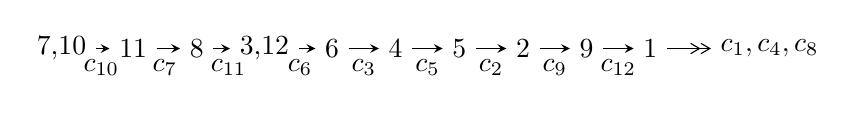
\begin{tikzpicture}[x=23pt, y=7pt]
	% node
	\node (A0) at (-1/8, 0) {7,10};
	\node (A1) at (1, 0) {11};
	\node (A2) at (2, 0) {8};
	\node (A3) at (49/16, 0) {3,12};
	\node (A4) at (33/8, 0) {6};
	\node (A5) at (41/8, 0) {4};
	\node (A6) at (49/8, 0) {5};
	\node (A7) at (57/8, 0) {2};
	\node (A8) at (65/8, 0) {9};
	\node (A9) at (73/8, 0) {1};
	\node (C1) at (1/2, -1) {$c_{10}$};
	\node (C2) at (3/2, -1) {$c_{7}$};
	\node (C3) at (5/2, -1) {$c_{11}$};
	\node (C4) at (29/8, -1) {$c_{6}$};
	\node (C5) at (37/8, -1) {$c_{3}$};
	\node (C6) at (45/8, -1) {$c_{5}$};
	\node (C7) at (53/8, -1) {$c_{2}$};
	\node (C8) at (61/8, -1) {$c_{9}$};
	\node (C9) at (69/8, -1) {$c_{12}$};
	\node (A10) at (11, 0) {$c_{1},c_{4},c_{8}$};

	% edge
	\draw[->,>=stealth]	
	(A0) edge (A1) (A1) edge (A2) (A2) edge (A3) (A3) edge (A4) (A4) edge (A5) (A5) edge (A6) (A6) edge (A7) (A7) edge (A8) (A8) edge (A9) ;
	\draw[->>,>={angle 60}]	
	(A9) edge (A10);
\end{tikzpicture} \\ 

\end{tabular} \\

\footnotetext{
The image of knot diagram is generated by the software ``\textbf{Draw programme}" developed by Andrew Bartholomew(\url{http://www.layer8.co.uk/maths/draw/index.htm\#Running-draw}), where we modified some parts for our purpose(\url{https://github.com/CATsTAILs/LinksPainter}).
}\phantom \\ \newline 
\centering \textbf{Ideals for irreducible components\footnotemark of $X_{\text{par}}$} 
 
\begin{align*}
I^u_{1}&=\langle 
237180958840 u^{40}+426640636409 u^{39}+\cdots+126602287463 b-603869550171,\\
\phantom{I^u_{1}}&\phantom{= \langle  }184156720841 u^{40}+260129939039 u^{39}+\cdots+379806862389 a-927659389454,\\
\phantom{I^u_{1}}&\phantom{= \langle  }u^{41}+2 u^{40}+\cdots-5 u-1\rangle \\
I^u_{2}&=\langle 
-2 u^4- u^3+b+u-3,\;a,\;u^5+u^4- u^2+u+1\rangle \\
\\
\end{align*}
\raggedright * 2 irreducible components of $\dim_{\mathbb{C}}=0$, with total 46 representations.\\
\footnotetext{All coefficients of polynomials are rational numbers. But the coefficients are sometimes approximated in decimal forms when there is not enough margin.}
\newpage
\renewcommand{\arraystretch}{1}
\centering \section*{I. $I^u_{1}= \langle 2.37\times10^{11} u^{40}+4.27\times10^{11} u^{39}+\cdots+1.27\times10^{11} b-6.04\times10^{11},\;1.84\times10^{11} u^{40}+2.60\times10^{11} u^{39}+\cdots+3.80\times10^{11} a-9.28\times10^{11},\;u^{41}+2 u^{40}+\cdots-5 u-1 \rangle$}
\flushleft \textbf{(i) Arc colorings}\\
\begin{tabular}{m{7pt} m{180pt} m{7pt} m{180pt} }
\flushright $a_{7}=$&$\begin{pmatrix}0\\u\end{pmatrix}$ \\
\flushright $a_{10}=$&$\begin{pmatrix}1\\0\end{pmatrix}$ \\
\flushright $a_{11}=$&$\begin{pmatrix}1\\u^2\end{pmatrix}$ \\
\flushright $a_{8}=$&$\begin{pmatrix}- u\\- u^3+u\end{pmatrix}$ \\
\flushright $a_{3}=$&$\begin{pmatrix}-0.484869 u^{40}-0.684901 u^{39}+\cdots+1.43981 u+2.44245\\-1.87343 u^{40}-3.36993 u^{39}+\cdots+10.8768 u+4.76982\end{pmatrix}$ \\
\flushright $a_{12}=$&$\begin{pmatrix}- u^2+1\\u^2\end{pmatrix}$ \\
\flushright $a_{6}=$&$\begin{pmatrix}0.839243 u^{40}+0.839308 u^{39}+\cdots-4.68096 u-0.119652\\-3.44624 u^{40}-3.41234 u^{39}+\cdots+13.1682 u+3.81213\end{pmatrix}$ \\
\flushright $a_{4}=$&$\begin{pmatrix}2.36382 u^{40}+2.16411 u^{39}+\cdots-7.95826 u+1.01795\\-5.33759 u^{40}-3.95656 u^{39}+\cdots+14.0481 u+5.35650\end{pmatrix}$ \\
\flushright $a_{5}=$&$\begin{pmatrix}-0.545392 u^{40}-0.945298 u^{39}+\cdots+1.68058 u+1.67265\\-2.45910 u^{40}-2.60458 u^{39}+\cdots+10.3453 u+3.00449\end{pmatrix}$ \\
\flushright $a_{2}=$&$\begin{pmatrix}0.605914 u^{40}+0.205696 u^{39}+\cdots-1.92135 u+3.09715\\-4.95524 u^{40}-5.16076 u^{39}+\cdots+18.1862 u+6.76084\end{pmatrix}$ \\
\flushright $a_{9}=$&$\begin{pmatrix}u^4- u^2+1\\- u^4\end{pmatrix}$ \\
\flushright $a_{1}=$&$\begin{pmatrix}- u^6+u^4-2 u^2+1\\u^6+u^2\end{pmatrix}$\\&\end{tabular}
\flushleft \textbf{(ii) Obstruction class $= -1$}\\~\\
\flushleft \textbf{(iii) Cusp Shapes $= -\frac{159607686408}{126602287463} u^{40}-\frac{572526761426}{126602287463} u^{39}+\cdots+\frac{127765468738}{126602287463} u+\frac{346980052385}{126602287463}$}\\~\\
\newpage\renewcommand{\arraystretch}{1}
\flushleft \textbf{(iv) u-Polynomials at the component}\newline \\
\begin{tabular}{m{50pt}|m{274pt}}
Crossings & \hspace{64pt}u-Polynomials at each crossing \\
\hline $$\begin{aligned}c_{1}\end{aligned}$$&$\begin{aligned}
&u^{41}+44 u^{40}+\cdots+2355 u+1
\end{aligned}$\\
\hline $$\begin{aligned}c_{2},c_{4}\end{aligned}$$&$\begin{aligned}
&u^{41}-6 u^{40}+\cdots+47 u-1
\end{aligned}$\\
\hline $$\begin{aligned}c_{3},c_{6}\end{aligned}$$&$\begin{aligned}
&u^{41}+7 u^{40}+\cdots+64 u+32
\end{aligned}$\\
\hline $$\begin{aligned}c_{5},c_{8}\end{aligned}$$&$\begin{aligned}
&u^{41}-2 u^{40}+\cdots+u-1
\end{aligned}$\\
\hline $$\begin{aligned}c_{7},c_{10}\end{aligned}$$&$\begin{aligned}
&u^{41}+2 u^{40}+\cdots-5 u-1
\end{aligned}$\\
\hline $$\begin{aligned}c_{9},c_{11},c_{12}\end{aligned}$$&$\begin{aligned}
&u^{41}+12 u^{40}+\cdots+9 u+1
\end{aligned}$\\
\hline
\end{tabular}\\~\\
\newpage\renewcommand{\arraystretch}{1}
\flushleft \textbf{(v) Riley Polynomials at the component}\newline \\
\begin{tabular}{m{50pt}|m{274pt}}
Crossings & \hspace{64pt}Riley Polynomials at each crossing \\
\hline $$\begin{aligned}c_{1}\end{aligned}$$&$\begin{aligned}
&y^{41}-88 y^{40}+\cdots+5466307 y-1
\end{aligned}$\\
\hline $$\begin{aligned}c_{2},c_{4}\end{aligned}$$&$\begin{aligned}
&y^{41}-44 y^{40}+\cdots+2355 y-1
\end{aligned}$\\
\hline $$\begin{aligned}c_{3},c_{6}\end{aligned}$$&$\begin{aligned}
&y^{41}+33 y^{40}+\cdots+49664 y-1024
\end{aligned}$\\
\hline $$\begin{aligned}c_{5},c_{8}\end{aligned}$$&$\begin{aligned}
&y^{41}+42 y^{39}+\cdots+9 y-1
\end{aligned}$\\
\hline $$\begin{aligned}c_{7},c_{10}\end{aligned}$$&$\begin{aligned}
&y^{41}-12 y^{40}+\cdots+9 y-1
\end{aligned}$\\
\hline $$\begin{aligned}c_{9},c_{11},c_{12}\end{aligned}$$&$\begin{aligned}
&y^{41}+36 y^{40}+\cdots+145 y-1
\end{aligned}$\\
\hline
\end{tabular}\\~\\
\newpage\flushleft \textbf{(vi) Complex Volumes and Cusp Shapes}
$$\begin{array}{c|c|c}  
\text{Solutions to }I^u_{1}& \I (\text{vol} + \sqrt{-1}CS) & \text{Cusp shape}\\
 \hline 
\begin{aligned}
u &= -0.809815 + 0.656518 I \\
a &= \phantom{-}0.18310 + 1.61197 I \\
b &= \phantom{-}2.10023 - 1.97578 I\end{aligned}
 & -1.37603 + 0.57854 I & -11.62960 + 0.13351 I \\ \hline\begin{aligned}
u &= -0.809815 - 0.656518 I \\
a &= \phantom{-}0.18310 - 1.61197 I \\
b &= \phantom{-}2.10023 + 1.97578 I\end{aligned}
 & -1.37603 - 0.57854 I & -11.62960 - 0.13351 I \\ \hline\begin{aligned}
u &= \phantom{-}0.934060 + 0.150205 I \\
a &= -0.18148 - 1.61697 I \\
b &= \phantom{-}0.203825 + 1.369510 I\end{aligned}
 & -3.38084 - 3.41544 I & -14.4142 + 7.4507 I \\ \hline\begin{aligned}
u &= \phantom{-}0.934060 - 0.150205 I \\
a &= -0.18148 + 1.61697 I \\
b &= \phantom{-}0.203825 - 1.369510 I\end{aligned}
 & -3.38084 + 3.41544 I & -14.4142 - 7.4507 I \\ \hline\begin{aligned}
u &= \phantom{-}0.940510\phantom{ +0.000000I} \\
a &= -1.80150\phantom{ +0.000000I} \\
b &= \phantom{-}0.154280\phantom{ +0.000000I}\end{aligned}
 & -5.56664\phantom{ +0.000000I} & -18.9570\phantom{ +0.000000I} \\ \hline\begin{aligned}
u &= -0.765786 + 0.781729 I \\
a &= -1.48698 + 0.38083 I \\
b &= \phantom{-}0.91217 + 1.53968 I\end{aligned}
 & \phantom{-}2.58614 - 2.24374 I & -5.47598 + 3.48781 I \\ \hline\begin{aligned}
u &= -0.765786 - 0.781729 I \\
a &= -1.48698 - 0.38083 I \\
b &= \phantom{-}0.91217 - 1.53968 I\end{aligned}
 & \phantom{-}2.58614 + 2.24374 I & -5.47598 - 3.48781 I \\ \hline\begin{aligned}
u &= \phantom{-}0.825264 + 0.768049 I \\
a &= -0.533792 - 0.264806 I \\
b &= -0.363252 - 0.579554 I\end{aligned}
 & \phantom{-}2.79960 - 1.79972 I & -4.96538 + 4.18830 I \\ \hline\begin{aligned}
u &= \phantom{-}0.825264 - 0.768049 I \\
a &= -0.533792 + 0.264806 I \\
b &= -0.363252 + 0.579554 I\end{aligned}
 & \phantom{-}2.79960 + 1.79972 I & -4.96538 - 4.18830 I \\ \hline\begin{aligned}
u &= \phantom{-}0.871525 + 0.715232 I \\
a &= \phantom{-}0.317178 - 0.359818 I \\
b &= \phantom{-}2.05567 + 2.91440 I\end{aligned}
 & \phantom{-}0.88954 - 2.73561 I & \phantom{-}12.1135 + 7.6213 I\\
 \hline 
 \end{array}$$\newpage$$\begin{array}{c|c|c}  
\text{Solutions to }I^u_{1}& \I (\text{vol} + \sqrt{-1}CS) & \text{Cusp shape}\\
 \hline 
\begin{aligned}
u &= \phantom{-}0.871525 - 0.715232 I \\
a &= \phantom{-}0.317178 + 0.359818 I \\
b &= \phantom{-}2.05567 - 2.91440 I\end{aligned}
 & \phantom{-}0.88954 + 2.73561 I & \phantom{-}12.1135 - 7.6213 I \\ \hline\begin{aligned}
u &= \phantom{-}0.710841 + 0.488347 I \\
a &= \phantom{-}0.458035 - 0.499819 I \\
b &= -0.032082 + 0.328781 I\end{aligned}
 & \phantom{-}1.44935 - 1.91021 I & -0.76032 + 4.38625 I \\ \hline\begin{aligned}
u &= \phantom{-}0.710841 - 0.488347 I \\
a &= \phantom{-}0.458035 + 0.499819 I \\
b &= -0.032082 - 0.328781 I\end{aligned}
 & \phantom{-}1.44935 + 1.91021 I & -0.76032 - 4.38625 I \\ \hline\begin{aligned}
u &= -0.923416 + 0.674039 I \\
a &= \phantom{-}1.66369 + 0.14363 I \\
b &= -0.43727 - 2.53225 I\end{aligned}
 & -1.74586 + 4.59945 I & -12.56472 - 5.90817 I \\ \hline\begin{aligned}
u &= -0.923416 - 0.674039 I \\
a &= \phantom{-}1.66369 - 0.14363 I \\
b &= -0.43727 + 2.53225 I\end{aligned}
 & -1.74586 - 4.59945 I & -12.56472 + 5.90817 I \\ \hline\begin{aligned}
u &= \phantom{-}1.118030 + 0.271471 I \\
a &= -0.17044 + 1.50981 I \\
b &= -0.89384 - 1.26952 I\end{aligned}
 & -11.21910 - 7.94660 I & -13.0997 + 5.5632 I \\ \hline\begin{aligned}
u &= \phantom{-}1.118030 - 0.271471 I \\
a &= -0.17044 - 1.50981 I \\
b &= -0.89384 + 1.26952 I\end{aligned}
 & -11.21910 + 7.94660 I & -13.0997 - 5.5632 I \\ \hline\begin{aligned}
u &= -0.720515 + 0.902697 I \\
a &= \phantom{-}1.42868 - 0.16952 I \\
b &= -0.66709 - 1.95032 I\end{aligned}
 & -3.31648 - 7.81279 I & -7.43198 + 3.38635 I \\ \hline\begin{aligned}
u &= -0.720515 - 0.902697 I \\
a &= \phantom{-}1.42868 + 0.16952 I \\
b &= -0.66709 + 1.95032 I\end{aligned}
 & -3.31648 + 7.81279 I & -7.43198 - 3.38635 I \\ \hline\begin{aligned}
u &= -1.121650 + 0.291198 I \\
a &= \phantom{-}0.498876 - 1.312020 I \\
b &= -1.197720 + 0.633604 I\end{aligned}
 & -11.09620 - 0.45608 I & -13.41842 - 0.76918 I\\
 \hline 
 \end{array}$$\newpage$$\begin{array}{c|c|c}  
\text{Solutions to }I^u_{1}& \I (\text{vol} + \sqrt{-1}CS) & \text{Cusp shape}\\
 \hline 
\begin{aligned}
u &= -1.121650 - 0.291198 I \\
a &= \phantom{-}0.498876 + 1.312020 I \\
b &= -1.197720 - 0.633604 I\end{aligned}
 & -11.09620 + 0.45608 I & -13.41842 + 0.76918 I \\ \hline\begin{aligned}
u &= -0.019251 + 0.828572 I \\
a &= -1.74001 + 0.53051 I \\
b &= \phantom{-}1.287330 - 0.377518 I\end{aligned}
 & -7.34491 + 4.27339 I & -8.31191 - 2.78880 I \\ \hline\begin{aligned}
u &= -0.019251 - 0.828572 I \\
a &= -1.74001 - 0.53051 I \\
b &= \phantom{-}1.287330 + 0.377518 I\end{aligned}
 & -7.34491 - 4.27339 I & -8.31191 + 2.78880 I \\ \hline\begin{aligned}
u &= \phantom{-}0.731013 + 0.924450 I \\
a &= \phantom{-}0.923425 + 0.604573 I \\
b &= -1.26483 + 1.04082 I\end{aligned}
 & -2.90816 - 0.63484 I & -9.12562 + 1.25059 I \\ \hline\begin{aligned}
u &= \phantom{-}0.731013 - 0.924450 I \\
a &= \phantom{-}0.923425 - 0.604573 I \\
b &= -1.26483 - 1.04082 I\end{aligned}
 & -2.90816 + 0.63484 I & -9.12562 - 1.25059 I \\ \hline\begin{aligned}
u &= -0.804662 + 0.114668 I \\
a &= -0.147294 + 0.641401 I \\
b &= \phantom{-}0.80950 - 2.46652 I\end{aligned}
 & -2.53010 + 0.33755 I & -19.6414 + 2.1587 I \\ \hline\begin{aligned}
u &= -0.804662 - 0.114668 I \\
a &= -0.147294 - 0.641401 I \\
b &= \phantom{-}0.80950 + 2.46652 I\end{aligned}
 & -2.53010 - 0.33755 I & -19.6414 - 2.1587 I \\ \hline\begin{aligned}
u &= \phantom{-}0.926559 + 0.745351 I \\
a &= \phantom{-}0.274837 + 0.567927 I \\
b &= -1.08422 - 1.33352 I\end{aligned}
 & \phantom{-}2.48539 - 3.92858 I & -5.87670 + 1.12171 I \\ \hline\begin{aligned}
u &= \phantom{-}0.926559 - 0.745351 I \\
a &= \phantom{-}0.274837 - 0.567927 I \\
b &= -1.08422 + 1.33352 I\end{aligned}
 & \phantom{-}2.48539 + 3.92858 I & -5.87670 - 1.12171 I \\ \hline\begin{aligned}
u &= -0.965249 + 0.735330 I \\
a &= \phantom{-}0.31200 - 1.49463 I \\
b &= -2.37280 + 1.50589 I\end{aligned}
 & \phantom{-}1.97721 + 7.97688 I & -7.20424 - 8.75185 I\\
 \hline 
 \end{array}$$\newpage$$\begin{array}{c|c|c}  
\text{Solutions to }I^u_{1}& \I (\text{vol} + \sqrt{-1}CS) & \text{Cusp shape}\\
 \hline 
\begin{aligned}
u &= -0.965249 - 0.735330 I \\
a &= \phantom{-}0.31200 + 1.49463 I \\
b &= -2.37280 - 1.50589 I\end{aligned}
 & \phantom{-}1.97721 - 7.97688 I & -7.20424 + 8.75185 I \\ \hline\begin{aligned}
u &= -0.930134 + 0.890297 I \\
a &= -0.321692 - 0.288040 I \\
b &= -0.267302 + 0.867780 I\end{aligned}
 & \phantom{-}9.70942 + 3.28933 I & \phantom{-}6.13928 - 1.45507 I \\ \hline\begin{aligned}
u &= -0.930134 - 0.890297 I \\
a &= -0.321692 + 0.288040 I \\
b &= -0.267302 - 0.867780 I\end{aligned}
 & \phantom{-}9.70942 - 3.28933 I & \phantom{-}6.13928 + 1.45507 I \\ \hline\begin{aligned}
u &= -1.037090 + 0.774259 I \\
a &= -0.100822 + 1.364460 I \\
b &= \phantom{-}2.50179 - 1.88429 I\end{aligned}
 & -4.3067 + 14.0138 I & -8.63515 - 7.83947 I \\ \hline\begin{aligned}
u &= -1.037090 - 0.774259 I \\
a &= -0.100822 - 1.364460 I \\
b &= \phantom{-}2.50179 + 1.88429 I\end{aligned}
 & -4.3067 - 14.0138 I & -8.63515 + 7.83947 I \\ \hline\begin{aligned}
u &= \phantom{-}1.045430 + 0.785315 I \\
a &= -0.491121 - 0.952641 I \\
b &= \phantom{-}2.29006 + 0.47538 I\end{aligned}
 & -3.90534 - 5.67266 I & -9.98188 + 3.51111 I \\ \hline\begin{aligned}
u &= \phantom{-}1.045430 - 0.785315 I \\
a &= -0.491121 + 0.952641 I \\
b &= \phantom{-}2.29006 - 0.47538 I\end{aligned}
 & -3.90534 + 5.67266 I & -9.98188 - 3.51111 I \\ \hline\begin{aligned}
u &= -0.666990\phantom{ +0.000000I} \\
a &= \phantom{-}0.215563\phantom{ +0.000000I} \\
b &= \phantom{-}0.523845\phantom{ +0.000000I}\end{aligned}
 & -0.906933\phantom{ +0.000000I} & -11.3940\phantom{ +0.000000I} \\ \hline\begin{aligned}
u &= -0.035730 + 0.419728 I \\
a &= \phantom{-}2.06556 - 0.62654 I \\
b &= -0.346501 - 0.304456 I\end{aligned}
 & -0.57624 + 1.50346 I & -4.65093 - 4.60849 I \\ \hline\begin{aligned}
u &= -0.035730 - 0.419728 I \\
a &= \phantom{-}2.06556 + 0.62654 I \\
b &= -0.346501 + 0.304456 I\end{aligned}
 & -0.57624 - 1.50346 I & -4.65093 + 4.60849 I\\
 \hline 
 \end{array}$$\newpage$$\begin{array}{c|c|c}  
\text{Solutions to }I^u_{1}& \I (\text{vol} + \sqrt{-1}CS) & \text{Cusp shape}\\
 \hline 
\begin{aligned}
u &= -0.332380\phantom{ +0.000000I} \\
a &= \phantom{-}1.68244\phantom{ +0.000000I} \\
b &= \phantom{-}1.85453\phantom{ +0.000000I}\end{aligned}
 & -2.28489\phantom{ +0.000000I} & \phantom{-}0.221560\phantom{ +0.000000I}\\
 \hline 
 \end{array}$$\newpage\newpage\renewcommand{\arraystretch}{1}
\centering \section*{II. $I^u_{2}= \langle -2 u^4- u^3+b+u-3,\;a,\;u^5+u^4- u^2+u+1 \rangle$}
\flushleft \textbf{(i) Arc colorings}\\
\begin{tabular}{m{7pt} m{180pt} m{7pt} m{180pt} }
\flushright $a_{7}=$&$\begin{pmatrix}0\\u\end{pmatrix}$ \\
\flushright $a_{10}=$&$\begin{pmatrix}1\\0\end{pmatrix}$ \\
\flushright $a_{11}=$&$\begin{pmatrix}1\\u^2\end{pmatrix}$ \\
\flushright $a_{8}=$&$\begin{pmatrix}- u\\- u^3+u\end{pmatrix}$ \\
\flushright $a_{3}=$&$\begin{pmatrix}0\\2 u^4+u^3- u+3\end{pmatrix}$ \\
\flushright $a_{12}=$&$\begin{pmatrix}- u^2+1\\u^2\end{pmatrix}$ \\
\flushright $a_{6}=$&$\begin{pmatrix}0\\u\end{pmatrix}$ \\
\flushright $a_{4}=$&$\begin{pmatrix}0\\2 u^4+u^3- u+3\end{pmatrix}$ \\
\flushright $a_{5}=$&$\begin{pmatrix}u^3\\- u^4- u^3+u^2-1\end{pmatrix}$ \\
\flushright $a_{2}=$&$\begin{pmatrix}- u^3\\3 u^4+2 u^3- u^2- u+4\end{pmatrix}$ \\
\flushright $a_{9}=$&$\begin{pmatrix}u^4- u^2+1\\- u^4\end{pmatrix}$ \\
\flushright $a_{1}=$&$\begin{pmatrix}- u^3\\u^4+u^3- u^2+1\end{pmatrix}$\\&\end{tabular}
\flushleft \textbf{(ii) Obstruction class $= 1$}\\~\\
\flushleft \textbf{(iii) Cusp Shapes $= -18 u^4-7 u^3+7 u^2+18 u-39$}\\~\\
\newpage\renewcommand{\arraystretch}{1}
\flushleft \textbf{(iv) u-Polynomials at the component}\newline \\
\begin{tabular}{m{50pt}|m{274pt}}
Crossings & \hspace{64pt}u-Polynomials at each crossing \\
\hline $$\begin{aligned}c_{1},c_{2}\end{aligned}$$&$\begin{aligned}
&(u-1)^5
\end{aligned}$\\
\hline $$\begin{aligned}c_{3},c_{6}\end{aligned}$$&$\begin{aligned}
&u^5
\end{aligned}$\\
\hline $$\begin{aligned}c_{4}\end{aligned}$$&$\begin{aligned}
&(u+1)^5
\end{aligned}$\\
\hline $$\begin{aligned}c_{5},c_{9}\end{aligned}$$&$\begin{aligned}
&u^5- u^4+4 u^3-3 u^2+3 u-1
\end{aligned}$\\
\hline $$\begin{aligned}c_{7}\end{aligned}$$&$\begin{aligned}
&u^5- u^4+u^2+u-1
\end{aligned}$\\
\hline $$\begin{aligned}c_{8},c_{11},c_{12}\end{aligned}$$&$\begin{aligned}
&u^5+u^4+4 u^3+3 u^2+3 u+1
\end{aligned}$\\
\hline $$\begin{aligned}c_{10}\end{aligned}$$&$\begin{aligned}
&u^5+u^4- u^2+u+1
\end{aligned}$\\
\hline
\end{tabular}\\~\\
\newpage\renewcommand{\arraystretch}{1}
\flushleft \textbf{(v) Riley Polynomials at the component}\newline \\
\begin{tabular}{m{50pt}|m{274pt}}
Crossings & \hspace{64pt}Riley Polynomials at each crossing \\
\hline $$\begin{aligned}c_{1},c_{2},c_{4}\end{aligned}$$&$\begin{aligned}
&(y-1)^5
\end{aligned}$\\
\hline $$\begin{aligned}c_{3},c_{6}\end{aligned}$$&$\begin{aligned}
&y^5
\end{aligned}$\\
\hline $$\begin{aligned}c_{5},c_{8},c_{9}\\c_{11},c_{12}\end{aligned}$$&$\begin{aligned}
&y^5+7 y^4+16 y^3+13 y^2+3 y-1
\end{aligned}$\\
\hline $$\begin{aligned}c_{7},c_{10}\end{aligned}$$&$\begin{aligned}
&y^5- y^4+4 y^3-3 y^2+3 y-1
\end{aligned}$\\
\hline
\end{tabular}\\~\\
\newpage\flushleft \textbf{(vi) Complex Volumes and Cusp Shapes}
$$\begin{array}{c|c|c}  
\text{Solutions to }I^u_{2}& \I (\text{vol} + \sqrt{-1}CS) & \text{Cusp shape}\\
 \hline 
\begin{aligned}
u &= \phantom{-}0.758138 + 0.584034 I \\
a &= \phantom{-0.000000 } 0 \\
b &= \phantom{-}0.442614 + 1.051550 I\end{aligned}
 & \phantom{-}0.17487 - 2.21397 I & -8.20462 + 3.60694 I \\ \hline\begin{aligned}
u &= \phantom{-}0.758138 - 0.584034 I \\
a &= \phantom{-0.000000 } 0 \\
b &= \phantom{-}0.442614 - 1.051550 I\end{aligned}
 & \phantom{-}0.17487 + 2.21397 I & -8.20462 - 3.60694 I \\ \hline\begin{aligned}
u &= -0.935538 + 0.903908 I \\
a &= \phantom{-0.000000 } 0 \\
b &= -0.304213 + 0.337334 I\end{aligned}
 & \phantom{-}9.31336 + 3.33174 I & -14.3260 - 3.4701 I \\ \hline\begin{aligned}
u &= -0.935538 - 0.903908 I \\
a &= \phantom{-0.000000 } 0 \\
b &= -0.304213 - 0.337334 I\end{aligned}
 & \phantom{-}9.31336 - 3.33174 I & -14.3260 + 3.4701 I \\ \hline\begin{aligned}
u &= -0.645200\phantom{ +0.000000I} \\
a &= \phantom{-0.000000 } 0 \\
b &= \phantom{-}3.72320\phantom{ +0.000000I}\end{aligned}
 & -2.52712\phantom{ +0.000000I} & -48.9390\phantom{ +0.000000I}\\
 \hline 
 \end{array}$$\newpage
\newpage\renewcommand{\arraystretch}{1}
\centering \section*{ III. u-Polynomials}
\begin{tabular}{m{50pt}|m{274pt}}
Crossings & \hspace{64pt}u-Polynomials at each crossing \\
\hline $$\begin{aligned}c_{1}\end{aligned}$$&$\begin{aligned}
&((u-1)^5)(u^{41}+44 u^{40}+\cdots+2355 u+1)
\end{aligned}$\\
\hline $$\begin{aligned}c_{2}\end{aligned}$$&$\begin{aligned}
&((u-1)^5)(u^{41}-6 u^{40}+\cdots+47 u-1)
\end{aligned}$\\
\hline $$\begin{aligned}c_{3},c_{6}\end{aligned}$$&$\begin{aligned}
&u^5(u^{41}+7 u^{40}+\cdots+64 u+32)
\end{aligned}$\\
\hline $$\begin{aligned}c_{4}\end{aligned}$$&$\begin{aligned}
&((u+1)^5)(u^{41}-6 u^{40}+\cdots+47 u-1)
\end{aligned}$\\
\hline $$\begin{aligned}c_{5}\end{aligned}$$&$\begin{aligned}
&(u^5- u^4+4 u^3-3 u^2+3 u-1)(u^{41}-2 u^{40}+\cdots+u-1)
\end{aligned}$\\
\hline $$\begin{aligned}c_{7}\end{aligned}$$&$\begin{aligned}
&(u^5- u^4+u^2+u-1)(u^{41}+2 u^{40}+\cdots-5 u-1)
\end{aligned}$\\
\hline $$\begin{aligned}c_{8}\end{aligned}$$&$\begin{aligned}
&(u^5+u^4+4 u^3+3 u^2+3 u+1)(u^{41}-2 u^{40}+\cdots+u-1)
\end{aligned}$\\
\hline $$\begin{aligned}c_{9}\end{aligned}$$&$\begin{aligned}
&(u^5- u^4+4 u^3-3 u^2+3 u-1)(u^{41}+12 u^{40}+\cdots+9 u+1)
\end{aligned}$\\
\hline $$\begin{aligned}c_{10}\end{aligned}$$&$\begin{aligned}
&(u^5+u^4- u^2+u+1)(u^{41}+2 u^{40}+\cdots-5 u-1)
\end{aligned}$\\
\hline $$\begin{aligned}c_{11},c_{12}\end{aligned}$$&$\begin{aligned}
&(u^5+u^4+4 u^3+3 u^2+3 u+1)(u^{41}+12 u^{40}+\cdots+9 u+1)
\end{aligned}$\\
\hline
\end{tabular}\newpage\renewcommand{\arraystretch}{1}
\centering \section*{ IV. Riley Polynomials}
\begin{tabular}{m{50pt}|m{274pt}}
Crossings & \hspace{64pt}Riley Polynomials at each crossing \\
\hline $$\begin{aligned}c_{1}\end{aligned}$$&$\begin{aligned}
&((y-1)^5)(y^{41}-88 y^{40}+\cdots+5466307 y-1)
\end{aligned}$\\
\hline $$\begin{aligned}c_{2},c_{4}\end{aligned}$$&$\begin{aligned}
&((y-1)^5)(y^{41}-44 y^{40}+\cdots+2355 y-1)
\end{aligned}$\\
\hline $$\begin{aligned}c_{3},c_{6}\end{aligned}$$&$\begin{aligned}
&y^5(y^{41}+33 y^{40}+\cdots+49664 y-1024)
\end{aligned}$\\
\hline $$\begin{aligned}c_{5},c_{8}\end{aligned}$$&$\begin{aligned}
&(y^5+7 y^4+16 y^3+13 y^2+3 y-1)(y^{41}+42 y^{39}+\cdots+9 y-1)
\end{aligned}$\\
\hline $$\begin{aligned}c_{7},c_{10}\end{aligned}$$&$\begin{aligned}
&(y^5- y^4+4 y^3-3 y^2+3 y-1)(y^{41}-12 y^{40}+\cdots+9 y-1)
\end{aligned}$\\
\hline $$\begin{aligned}c_{9},c_{11},c_{12}\end{aligned}$$&$\begin{aligned}
&(y^5+7 y^4+16 y^3+13 y^2+3 y-1)(y^{41}+36 y^{40}+\cdots+145 y-1)
\end{aligned}$\\
\hline
\end{tabular}
\vskip 2pc
\end{document}